% v4 Results part C: advancing the state (register R10-R13). Resolves the
% v3 operator confound (C1) with the shared-REX protocol; direct vs
% autoregressive; the conditioning null with seed bands (T2 correction).

\subsubsection{Advancing the state: forecasting without an oracle}
\label{sec:res_forecast}

The family ordering survives an operator-robust protocol, which resolves
the operator confound the suited-operator comparison of
\S\ref{sec:methods_closure} left open: one \DirectFC{}
(\S\ref{sec:methods_rex}), trained identically on each family's frozen
latents, is stable on every latent including the reconstructive ones. Under
it the predictive states are the more forecastable, decoded lift
$R^2 = \RexFamClw{}$ for the \PredState{} and \RexFamCln{} for the \LiftState{} against
\RexFamAeLw{} for the reconstructive anchor, three operator-training seeds
per family on the \TestSplit{} set, with the \LiftState{} latents the most forecastable of all
(figure~\ref{fig:forecast}a). The ordering agrees with the suited-operator
protocol, so it is a property of the states, not of the operator that
reads them.

The forecasting mechanism is the direct-versus-autoregressive contrast.
Rolled autoregressively through the impact, the matched transformer
compounds its own errors: forty steps from the pre-impact context its
decoded lift closes at \ArFortyClw{} on the \PredState{} latents and
\ArFortyCln{} on the \LiftState{} latents. The \DirectFC, emitting all forty steps in
one shot from the same context, closes at \RexTunedCl{} on the identical
protocol (figure~\ref{fig:forecast}b): rollout compounding, not the state,
is the failure mode. The direct forecast is a conditional median, and the
honest reading is that of a median: it contracts toward the climatology of
the shedding cycle where the encounter is unresolved, which is precisely
the model-error regime the assimilation of \S\ref{sec:res_da} must
correct.

Knowing the gust does not help. Conditioning the forecaster on the true
episode parameters $(G, D, Y)$, an oracle no deployment has, degrades the
forecast in every one of three operator seeds, \PoneCovOracle{} against
\PoneCovNone{} unconditioned, with non-overlapping seed bands: at the
present case count the oracle covariates overfit held-out parameter
combinations. A deployable phase covariate is a wash within seed noise
(\PoneCovPhase). This closes the estimation thesis from the third side:
forecast alone contracts, parameter oracles hurt, and what remains is the
model-plus-pressure route of part D.

\begin{figure}
  \centering
  \begin{subfigure}{\linewidth}
    \centering
    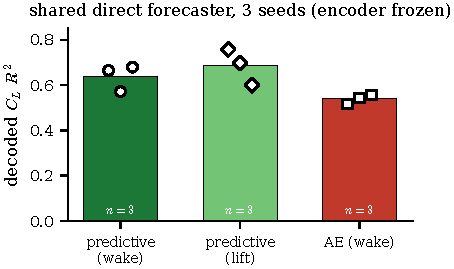
\includegraphics[width=0.92\linewidth]{sections/figures/results/fig_forecastability_v4.pdf}
    \caption{}
  \end{subfigure}
  \\[1.2ex]
  \begin{subfigure}{\linewidth}
    \centering
    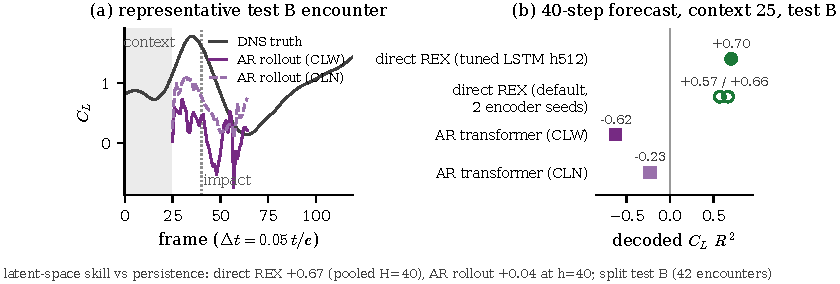
\includegraphics[width=0.92\linewidth]{sections/figures/results/fig_forecast40_v4.pdf}
    \caption{}
  \end{subfigure}
  \caption{Forecasting the state on the \TestSplit{} set. (a)~Decoded lift $R^2$ of the
  shared \DirectFC{} per family (three operator seeds each, bars at
  the seed mean) and the conditioning null (three seeds per arm): the
  $(G, D, Y)$ oracle degrades the forecast, the phase covariate is a wash.
  (b)~Direct versus autoregressive over forty steps through the impact
  from a $25$-frame context: the one-shot forecast stays usable where the
  rollout compounds.}
  \label{fig:forecast}
\end{figure}
